
\section{Experiment}
\label{cp3:experiment}



To investigate which text within a natural language artifact software developers deem as relevant to a task,
 we decide for a controlled experiment
 as it allows us to investigate the behavior of multiple developers
over a consistent set of artifacts.



In the experiment, detailed in the following subsections,
we asked 20 participants to highlight portions of a curated
set of artifacts relevant to completing six different development tasks;
 highlighting was followed by post-experiment 
interviews to understand the
strategies that participants employed to identify relevant text,
providing us both 
quantitive data (in the form of the highlights produced) 
and qualitative data (in the form of the interview transcripts) 
which we use to answer the research questions 
presented earlier in this chapter.






\acs{UBC} Behavioural Research Ethics Board  approved this experiment under the certificate \textit{H18-02104}.
The experiment's supplementary material is also publicly available~\cite{cp3_supplementary_material}.




\subsection{Tasks}
\label{cp3:method-tasks}


The six tasks in our experiment provide for a variety of information-seeking activities observed from earlier
studies, which include when a developer
refers to API documentation or Q\&A websites for API usage purposes~\cite{umarji2008archetypal, Singer1998,robillard2011field};
evaluates a possible reusable library to be incorporated into their implementation~\cite{umarji2008archetypal}; or
confirms a system's behaviour referring to past discussions in community forums or in the system's documentation~\cite{umarji2008archetypal, Lotufo2012, Singer1998}.
To design tasks for these activities, we applied criteria described by Petrosyan and colleagues~\cite{Petrosyan2015}, namely that
tasks must encompass common application domains and that the tasks' artifacts must be publicly available.


Table~\ref{tbl:tasks-overview-cp3} outlines the tasks designed.
For each task, the table provides a brief description and the task name, which refers to an identifier pertaining the topic or the system related to the task.
From this point forward, we will refer to the tasks according to these identifiers.
\texttt{Bugzilla} and \texttt{Yargs} are API usage tasks; \texttt{Networking} and \texttt{Databases} ask participants to evaluate and decide upon the adoption of a certain technology or framework; and finally, \texttt{GPMDPU} and \texttt{Lucene} describe scenarios where a participant 
has to understand the system's behaviour. 


Our decision to use a number of different systems employing
a variety of technologies aims to minimize the effects that might result from a participant being
well-acquainted with a particular system or technology~\cite{Wildemuth2012, DeGraaf2014}. 



\begin{table}
\caption{Tasks overview}
\begin{scriptsize}
\vspace{-1mm}  


\begin{threeparttable}    
\rowcolors{2}{}{lightgray}
\begin{tabular}{ll}
\hline    
\textbf{Task} & \textbf{Description} \\ 
\hline
\hline
Bugzilla & 
\parbox[l][0.9cm][c]{11cm}{Locate information about Bugzilla's REST API custom fields and how they can be included as part of the \texttt{GET /rest/bug} payload}  \\
%
Databases & 
\parbox[l][0.9cm][c]{11cm}{Review Q\&A forums and decide between the adoption of ORM or JDBC for a system's database being migrated from C to Java}  \\ 
%
GPMDPU & 
\parbox[l][0.9cm][c]{11cm}{Locate constraints or limitations about the GPMDPU shortcuts feature in order to work in a patch for this feature}  \\
%
Lucene & 
\parbox[l][0.9cm][c]{11cm}{Review the Lucene documentation and bug reports to understand how it computes similarity scores during indexing, particularly the BM25 score function, such that you can address a change request} \\
%
Networking & 
\parbox[l][0.9cm][c]{11cm}{Review the MDN documentation and Q\&A forums to decide between the adoption of Server-sent events or WebSockets technologies for a notification system being developed using Javascript } \\ 
%
Yargs & 
\parbox[l][1.2cm][c]{11cm}{Review the Yargs documentation and bug reports to check whether the API provides support for parsing mutually exclusive arguments, which is a requirement for a command line tool being developed in Python } \\
\hline
\end{tabular}
\end{threeparttable}    
\end{scriptsize}
\smallskip
\label{tbl:tasks-overview-cp3}
\end{table}




\subsection{Artifacts}
\label{cp3:method-artifacts}



For each task, we also needed to choose a set of artifacts for a
participant to peruse for relevant information to the task.  Based on
observations about the most common information sources sought in
development tasks~\cite{Li2013, Ponzanelli2017},
we focused on API documentation, Q\&A websites, and
bug reports.
For each task, a participant should consider on average three artifacts extracted
from one or more information sources.
We describe selection criteria for the artifacts and information sources as follows.


% \footnote{
% e.g.: https://www.google.com/search?q=bugzilla+REST+API
% }

To select the artifacts, for each task, we performed
searches and inspected the top 10 results retrieved by Google search engine, Stack Overflow, and in a
system's bug tracking system to select a set of candidate artifacts that could
assist in task completion.
For some tasks, the list of candidate
artifacts contained a single kind of artifact (e.g., bug
reports). For others, multiple kinds of candidate artifacts applied
(e.g., API documentation and Q\&A websites). 
Due to the varied availability of artifact types per task, 
we ensured that across
the six tasks, each kind of artifact appeared in at least half of the
tasks.



To produce the curated set of artifacts for each task, we then carefully read each candidate artifact.
Selection criteria considered an artifact's content and possible effects that 
could arise from interacting with a piece of text:
(1) strengthening an assumption, (2) contradicting or eliminating an assumption, or 
(3) combining multiple pieces of text to yield a conclusion~\cite{clark2013relevance}.
As examples of these criteria in action, the \texttt{Lucene}
artifacts chosen contain
complementary sources where sentences in different artifacts
pertain to the same topic
while the artifacts chosen for
the \texttt{GPMDPU} task contain contradictory information; two bug reports
argue that a feature is not supported while a third states otherwise.

We also asked two other software engineering researchers to provide a
list of candidate artifacts for each task based on the task's
description.  The Fleiss's Kappa coefficient score indicates a
moderate agreement level ($\kappa = 0.45$)~\cite{fleisskappa1977,
fleiss1981} on the list of provisioned resources suggesting that a
developer searching for pertinent artifacts for such tasks would
likely obtain a similar list of artifacts for inspection.



Table~\ref{tbl:corpus-stats} reports on the 20 artifacts used for the
experiment: 10 are documents describing APIs, 5 are bug reports, and 5
are Q\&A forum entries. These documents comprise nearly 1874
sentences and the average reading time~\cite{Just1980} of all artifacts of each task
is equivalent to 18.3 minutes ($\pm 5.5$ minutes). 





\begin{table}
\caption{Corpus overview}
\begin{footnotesize}
\begin{center}
% \begin{threeparttable} 
\rowcolors{2}{}{lightgray}
\begin{tabular}{l|cccccccc}
\hline    
\textbf{Task} 
&  \textbf{\# participants}
&   \textbf{\# Artifacts} 
&   \textbf{API} 
&   \textbf{Bugs} 
&   \textbf{Q\&A} 
&  \textbf{\# Sentences} \\ 
\hline    
\hline
Bugzilla    & 18 & 3 & 3 & 0 & 0 & 459 \\
Databases   & 17 & 3 & 0 & 0 & 3 & 232 \\
GPMDPU      & 18 & 3 & 0 & 3 & 0 & 291 \\
Lucene      & 15 & 3 & 2 & 1 & 0 & 170 \\     
Networking  & 17 & 5 & 4 & 0 & 1 & 313 \\
Yargs       & 18 & 3 & 1 & 1 & 1 & 409 \\
\hline    
\hline 
\rowcolor{white}
Total       & 20 & 20 & 10 & 5 & 5 & 1874  \\
\hline 
\end{tabular}
% \begin{tablenotes}
% \end{tablenotes}   
% \end{threeparttable} 
\end{center}
\end{footnotesize}
\label{tbl:corpus-stats}
\end{table}




\subsection{Participants}
\label{cp3:method-participants}


Twenty participants (2 self-identified as female and 18 as male) were recruited through
mailing lists for computer science graduate students 
and through personal contacts. To ensure participants were
familiar with concepts integral to the experiment, a demographic
survey included questions about the use of software documentation and
bug tracking systems by a participant.  No participants were excluded
based on answers to these questions.
Participants were compensated (\$20) for their participation.
At the time of the experiment, 5 participants were working as software
developers and 15 were graduate
students, of which 73\% have
previous professional experience. 
On average, participants self-reported 8.9 years of
programming experience ({\small $\pm$} 4, ranging from 3 to 20 years)
and 16 out of the 20 participants reported professional experience with an average of 4.7 years ({\small $\pm$}
3.7, ranging from 1 to 15 years).



\subsection{Procedures}
\label{cp3:procedures}



Each experimental session lasted no more than two hours; this length
of time was selected based on three pilot sessions.
We describe the final experimental set-up, referring to
changes made based on the pilot sessions.



Each session began with a short tutorial explaining the
experiment's purpose and describing how to use a provided tool (in
the form of a browser extension) to
highlight text relevant to a given task.
The concept of relevance was left to a participant's judgment as any
definition or explanation could introduce bias.
Each participant was able to practice use of the
tool on an example that was separate from the experimental tasks and
artifacts. We added this description of the tool and ability to 
practice with the tool after the first two pilot sessions. 


Participants worked on the assigned tasks in a given order and were
not required to complete all tasks.
We randomized the order of presentation of each task across
participants while also balancing the order of tasks~\cite{wohlin2012},
such that every task was first seen by an equal number of participants. 
Participants took as much time as they needed to complete a task.


For each task, a participant was presented with a description of the task in a PDF
viewer. The description included links to the artifacts a participant
was asked to consider as part of the task: when a link was followed,
the artifact would appear in a browser window.
A participant could choose to
consider the artifacts in any order and was asked to highlight any
text the participant considered relevant to complete the task.




When the participant
indicated completion of the task, a short questionnaire was
provided, specific for the task, that gathered background
information about a participant's knowledge related to the task
and whether they had likely gained appropriate knowledge
of how to complete the task. 
As an example, Figure~\ref{fig:networking-questions} provides an 
excerpt of the questionnaire presented for the \texttt{Networking} task.
% The questionnaire contains a five-level Likert scale~\cite{likert1932technique}
% for the familiarity and difficulty questions as well as likely solutions for the task. 


\begin{figure}
\begin{mdframed}[backgroundcolor=gray!15] 
\begin{scriptsize}

\noindent On a scale of 1 to 5, how familiar are you with the task's technologies: \smallskip

\quad \textit{(not at all familiar)} ~$1$ - $2$ - $3$ - $4$ - $5$ ~\textit{(extremely familiar)} 

\noindent\rule{8cm}{0.4pt} \smallskip

\noindent On a scale of 1 to 5, what was the level of difficulty of the task: \smallskip

\quad \textit{(very easy)} ~$1$ - $2$ - $3$ - $4$ - $5$ ~\textit{(very hard)} 

\noindent\rule{8cm}{0.4pt} \smallskip

\noindent Please evaluate the following sentences and mark only correct statements: \smallskip

\noindent $\square$ SSE are bidirectional and it can be used for pushing notifications to the bill-sharing system; \smallskip

\noindent $\square$ SSE works over HTTP with no additional components; \smallskip
    
\noindent $\square$ WebSockets are bidirectional and it can be used for pushing notifications to the bill-sharing system; \smallskip
    
\noindent $\square$ There are no data type limitations for SSE messages; \smallskip
    
\noindent $\square$ There are no data type limitations for WebSockets messages; \smallskip

\noindent\rule{8cm}{0.4pt} \smallskip

\noindent $\square$ WebSockets should be adopted for the notification system; \smallskip

\noindent $\square$ SSE should be adopted for the notification system; \smallskip

\noindent\rule{8cm}{0.4pt} \smallskip

\noindent $\square$ After reviewing the documentation, I don't have enough knowledge to complete this task

\end{scriptsize}
\end{mdframed}
\caption{Questionnaire for the Networking task asking about previous knowledge, expertise and likely solutions for the task}
\label{fig:networking-questions}
\end{figure}

    



Each session concluded with a debrief session where we discussed the
correctness of every task,
and also conducted a semi-structured
interview that discussed how a participant reasoned about relevance
and what features of the text, in their opinion, helped in deciding
whether information in the text was relevant or not.
To ensure that the session would finish in the allotted time,
we shortened the debriefing and interview components 
for certain participants
(e.g., as when a participant finished 4 tasks near the allotted time)
such that the study would not take longer than the stipulated 2 hours time period.
Overall, 11 out of the 20 participants completed all the tasks.
Table~\ref{tbl:corpus-stats} discriminates the number of participants who completed a task.




\subsection{Summary of Procedures}


We have described experimental procedures that allow us to inspect the 
text that 20 participants deemed relevant to different kinds of artifacts 
associated with six information-seeking tasks. 
Figure~\ref{fig:task-highlights-heatmap} illustrates the data gathered with this experiment. 
It shows a portion of a task description used in the experiment (left-side) and it
provides an overview of highlights (right-side) selected by
participants using our highlighting tool.



% \medskip
\begin{figure}
    \centering
    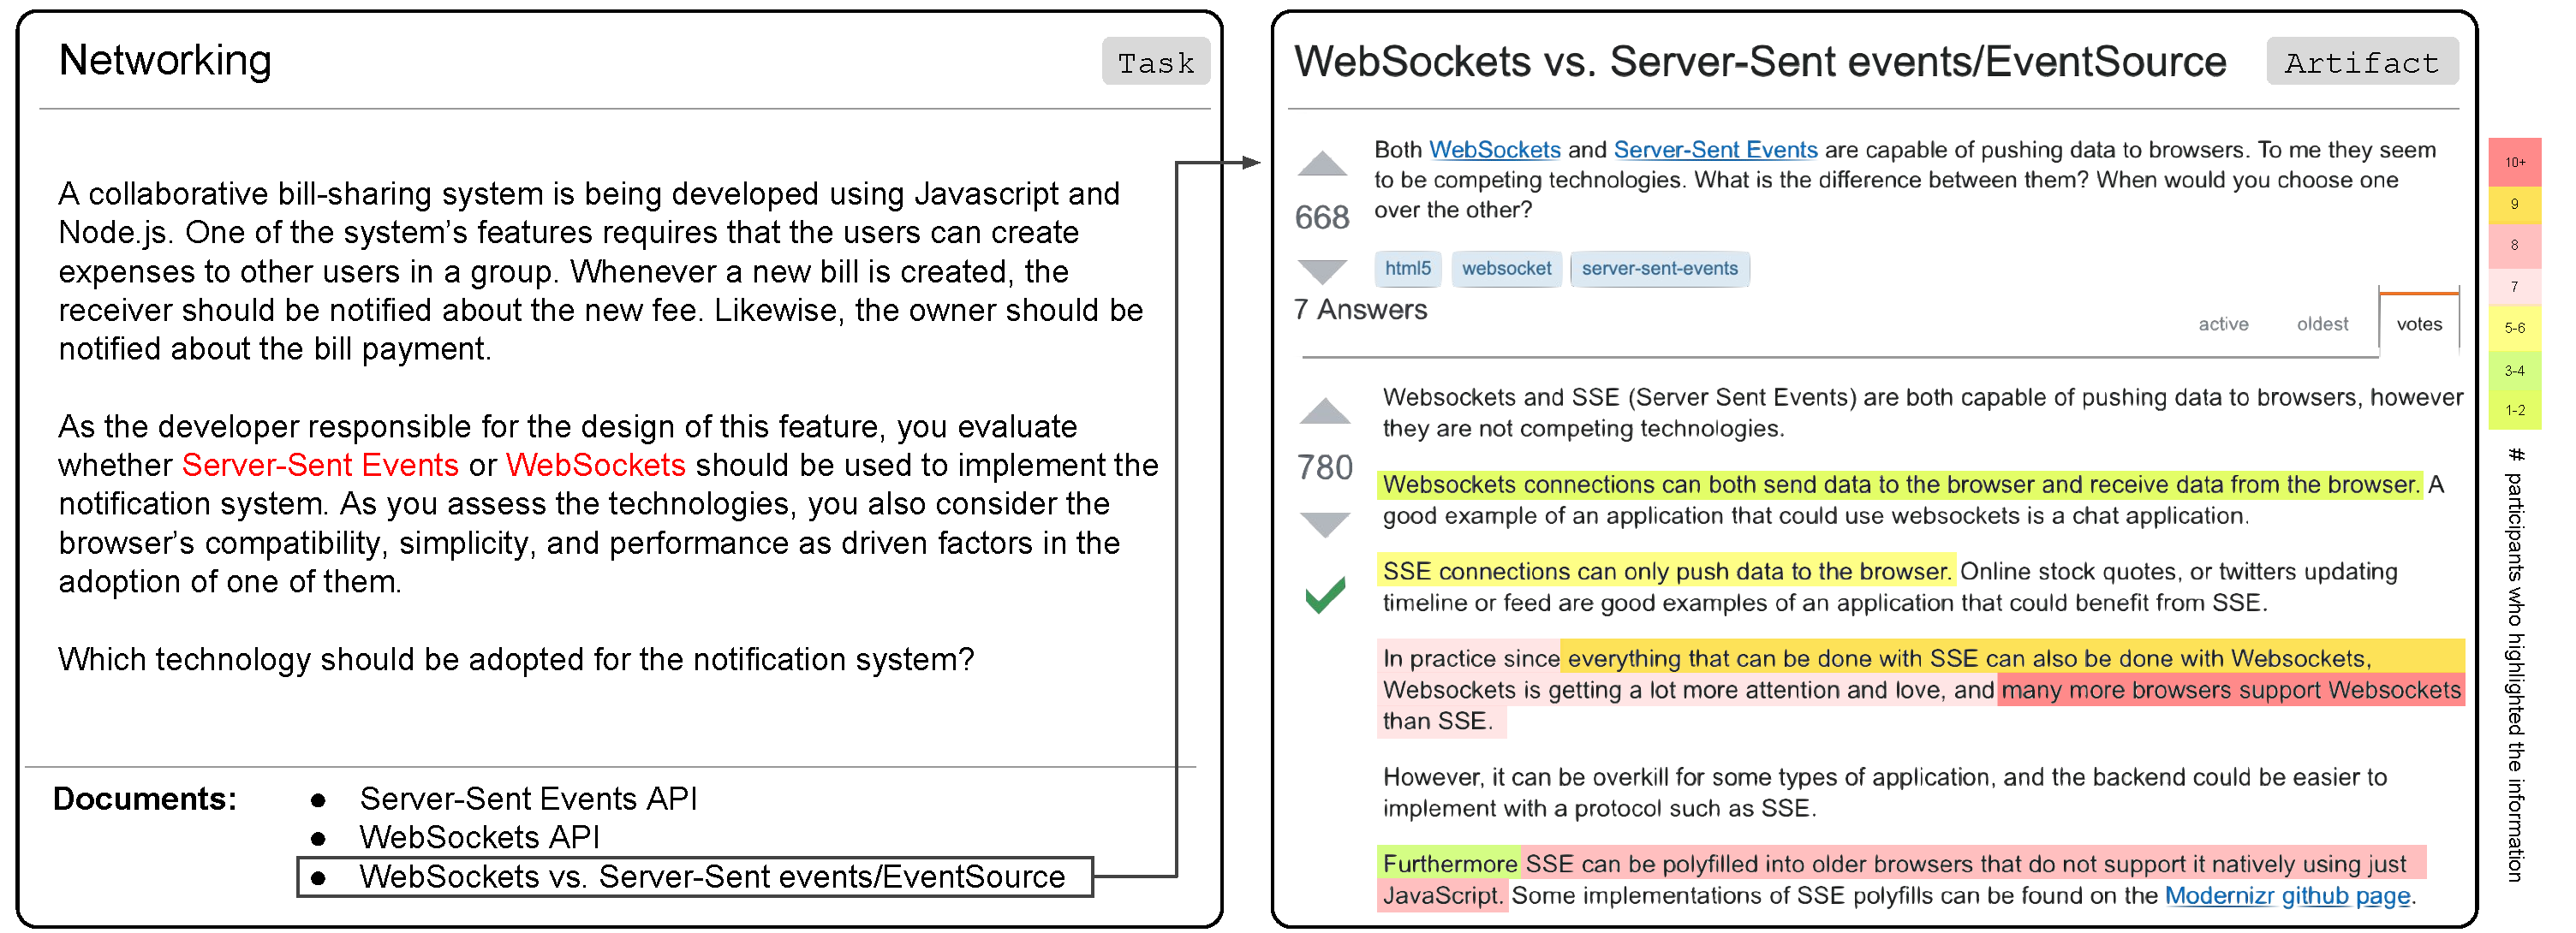
\includegraphics[width=1\textwidth]{cp3/heatmap}
\caption{An example of a task description and a depiction of collected data, shown as a heatmap of text that participants highlighted as relevant to the task}
\label{fig:task-highlights-heatmap}
\end{figure}
% \end{landscape}







